%This is a very basic  BE PROJECT PRELIMINARY template.

%#############################################
%#########Author :  PROJECT###########
%#########COMPUTER ENGINEERING############


\documentclass[oneside,a4paper,12pt]{report}
%\usepackage{showframe}
%\hoffset = 8.9436619718309859154929577464789pt
%\voffset = 13.028169014084507042253521126761pt

\fancypagestyle{plain}{%
  \fancyhf{}
  \fancyfoot[CE]{College_Name, Department of Computer Engineering 2015}
  \fancyfoot[RE]{\thepage}
}
\pagestyle{fancy}
\fancyhead{}
\renewcommand{\headrulewidth}{0pt}
\footskip = 0.625in
\cfoot{}
\rfoot{}

\usepackage[]{hyperref}
\usepackage{tikz}
\usetikzlibrary{arrows,shapes,snakes,automata,backgrounds,petri}

\usepackage{tabularx}

%\usepackage[nottoc,notlot,notlof,numbib]{tocbibind}
\usepackage[titletoc]{appendix}
\usepackage{titletoc}
\renewcommand{\appendixname}{Annexure}
\renewcommand{\bibname}{References}

\setcounter{secnumdepth}{5}

\usepackage{float}
\usepackage{subcaption}
\usepackage{multirow}

\usepackage[ruled,vlined]{algorithm2e}

\usepackage{amssymb}

\begin{document}
\setlength{\parindent}{0mm}
\begin{center}
% \vspace*{1\baselineskip}
{\bfseries A  PROJECT REPORT ON \\}
 \vspace*{2\baselineskip}
{\bfseries \fontsize{16}{12} \selectfont Astronomical Image colorization and super-resolution using GANs \\ \vspace*{2\baselineskip}}
{\fontsize{12}{12} \selectfont SUBMITTED TOWARDS THE
 \\PARTIAL FULFILMENT OF THE REQUIREMENTS OF \\

\vspace*{2\baselineskip}}
{\bfseries \fontsize{14}{12} \selectfont BACHELOR OF ENGINEERING (Computer
Engineering) \\
\vspace*{1\baselineskip}}
{\bfseries \fontsize{14}{12} \selectfont BY \\
\vspace*{1\baselineskip}}
Shreyas Kalvankar  \hspace{25 mm} Exam No:  \\
Hrushikesh Pandit \hspace{25 mm} Exam No:   \\
Pranav Parwate \hspace{30 mm} Exam No:  \\
Atharva Patil \hspace{34 mm} Exam No:\\
\vspace*{2\baselineskip}
{\bfseries \fontsize{14}{12} \selectfont Under The Guidance of \\
\vspace*{2\baselineskip}}
Prof. Dr. S.M. Kamalapur\\

\includegraphics[width=100pt]{collegelogo.png} \\
{\bfseries \fontsize{14}{12} \selectfont Department of Computer Engineering \\
K. K. Wagh Institute of Engineering Education \& Research \\
Hirabai Haridas Vidyanagari, Amrutdham, Panchavati, Nashik-422003 \\
Savitribai Phule Pune University\\
A. Y. 2020-21 Sem I
}
\end{center}

\newpage



\begin{figure}[ht]
\centering

\includegraphics[width=100pt]{collegelogo.png}
\end{figure}


{\bfseries \fontsize{14}{12} \selectfont \centerline{K. K. Wagh Institute of Engineering Education and Research}
\centerline{Department of Computer Engineering}
\vspace*{3\baselineskip}}


{\bfseries \fontsize{16}{12} \selectfont \centerline{CERTIFICATE}
\vspace*{3\baselineskip}}

\centerline{This is to certify that the Project Titled}
\vspace*{1\baselineskip}


{\bfseries \fontsize{14}{12} \selectfont \centerline{Astronomical Image colorization and super-resolution using GANs}
\vspace*{1\baselineskip}}

\centerline{Submitted by}
\vspace*{1\baselineskip}
\centerline{Shreyas Kalvankar  \hspace{25 mm} Exam No: }
\centerline{Hrushikesh Pandit \hspace{25 mm} Exam No:  }
\centerline{Pranav Parwate \hspace{30 mm} Exam No: }
\centerline{Atharva Patil \hspace{34 mm} Exam No: }
\vspace*{1\baselineskip}
is a bonafide work carried out by Students under the supervision of Prof. Dr. S.M. Kamalapur and it
is submitted towards the partial fulfilment of the requirement of Bachelor of Engineering (Computer Engineering) Project during academic year 2020-21.\\\\\\

\bgroup
\def\arraystretch{0.7}
\begin{tabular}{c c }
Prof. Dr. S.M. Kamalapur &  \hspace{25 mm} Prof. Dr. S. S. Sane \\
Internal Guide   &  \hspace{25 mm} Head \\
Department of Computer Engineering  &	\hspace{25 mm}Department of Computer Engineering  \\
\end{tabular}
%}



\newpage

%\pictcertificate{TITLE OF BE PROJECT}{Student Name}{Exam Seat No}{Guide Name}
\setcounter{page}{0}
\frontmatter
\cfoot {
\color{gray}
\scriptsize KKWIEER, Department of Computer Engineering 2019}
\rfoot{\thepage}
\pagenumbering{Roman}
%\pictack{BE PROJECT TITLE}{Guide Name}


{  \newpage {\bfseries \fontsize{14}{12} \selectfont \centerline{Abstract}
\vspace*{2\baselineskip}} \setlength{\parindent}{11mm} }
{ \setlength{\parindent}{0mm} }
\hspace*{0.25 in}Automated colorization of black and white images has been subject to much research within the computer vision and machine learning communities. Beyond simply being fascinating from an aesthetic and artificial intelligence perspective, such capability has broad practical applications. It is an area of research that possesses great potentials in applications: from black and white photo reconstruction, image augmentation, video restoration to image enhancement for improved interpretability.\\
\hspace*{0.25 in}Image downscaling is an innately lossy process. The principal objective of super resolution imaging is to reconstruct a low resolution image into a high resolution one based on a set of low-resolution images to rectify the limitations that existed while the procurement of the original low-resolution images. This is to insure better visualization and recognition for either scientific or non-scientific purposes. No matter how good an upscaling algorithm is, there will always be some amount of high frequency data lost from a downscale-upscale function performed on the image. Ultimately, even the best upscaling algorithms cannot effectively reconstruct data that does not exist. Traditional methods for image upsampling rely on low-information, smooth interpolation between known pixels. Such methods can be treated as a convolution with a kernel encoding no information about the original image. A solution to the problem is by using Generative Adversarial Networks (GANs) to hallucinate high-frequency data in a super-resolved image that does not exist in the smaller image. Although they increase the resolution of an image, they fail to produce the clarity desired in the super-resolution task. By using the above mentioned method, not a perfect reconstruction can be obtained albeit instead a rather plausible guess can be made at what the lost data might be, constrained to reality by a loss function penalizing deviations from the ground truth image.
\hspace*{0.25 in}A huge number of raw images lie unprocessed and unseen in the Hubble Legacy Archives. These raw images are typically low-resolution, black and white and unfit to be shared with the world. It takes huge amounts of hours to process them. This processing is necessary because astronomers often struggle to distinguish objects from the raw images. Random and synthetic noise from the sensors in the telescope, changing optical characteristics in the system and noise from other bodies in the universe all make the processing further necessary. Furthermore, colorization is needed to help highlight small features that ordinarily wouldn't be able to be picked out against noise of the image. The processing of the images is so time consuming that the images are rarely seen by human eyes. The problem is only likely to get worse. Not only is new data being continuously produced by Hubble Telescope, but new telescopes are soon to come online. A simplification of image processing by using artificial image colorization and super-resolution can be done in an automated fashion to make it easier for astronomers to visually identify and analyze objects in Hubble dataset.

{  \newpage {\bfseries \fontsize{14}{12} \selectfont \centerline{Acknowledgments}
\vspace*{2\baselineskip}} \setlength{\parindent}{11mm} }
{ \setlength{\parindent}{0mm} }
please enter text here.\\
\vspace*{3\baselineskip} \\
\begin{tabular}{p{8.2cm}c}
&Shreyas Kalvankar\\
&Hrushikesh Pandit\\
&Pranav Parwate\\
&Atharva Patil\\
&(B.E. Computer Engg.)
%}
\end{tabular}


% \maketitle
\tableofcontents
\listoffigures
\listoftables



\mainmatter



  \titleformat{\chapter}[display]
{\fontsize{16}{15}\filcenter}
{\vspace*{\fill}
 \bfseries\LARGE\MakeUppercase{\chaptertitlename}~\thechapter}
{1pc}
{\bfseries\LARGE\MakeUppercase}
[\thispagestyle{empty}\vspace*{\fill}\newpage]







\setlength{\parindent}{11mm}





\chapter{Introduction}
\section{Project Idea}
\begin{itemize}
\item The idea of the project is to create a efficient mathematical model for image colorization and super resolution using Generative Adversarial Networks (GANs)
\item Having two networks compete will stimulate greater performance by the virtue of minimization of loss functions that traditional Convolutional Neural Network cant do
\end{itemize}


\section{Motivation of the Project}
\begin{itemize}
\item Image colorization seems to be evolving as computers get better and better at predicting missing variables. Different methods and techniques have been applied for colorizing images that have shown promising results
\item Introduction of convolutional neural networks has made this task even more precise and accurate. Convoluting grayscale images to RGB provides unprecedented results with reference to visual inspection
\item With the introduction of Generative Adversarial Networks, this particular task can be developed and modified to increase the efficiency and precision for colorizing images instead
\item Furthermore, image upscaling is another problem that has been under research in the computer vision community. It has been studied and many approached have been developed to accurately predict the missing pixel values while upscaling an image
\item Application of GANs to this discipline has successfully improved the performance and computers are getting better and better at predicting accurate missing pixel values and upscaling images many folds the original size
\item All this computation power can be used for astronomical research by processing large data archives
\item A large number of images lie dormant in most of the space survey data archives which never go through any kind of processing and are low resolution and black \& white. These images could be processed automatically by an algorithm that will colorize and super-resolve the images which can make it easier for astronomers to visually inspect the images
\end{itemize}

\section{Literature Survey}
\subsection{Image Colorization}
\subsubsection{Hint Based Colorization}
\hspace*{0.25 in}\cite{levin2004colorization} proposed using colorization hints from the user in a quadratic cost function which imposed that neighboring pixels in space-time with similar intensities should have similar colours. This was a simple but effective method but only had hints which were provided in form of imprecise colored scribbles on the grayscale input image. But with no additional information about the image, the method was able to efficiently generate high quality colorizations. \cite{huang2005edge} addressed the color bleeding issue faced in this approach and solved it using adaptive edge detection. \cite{yatziv2006chrominance} used luminescence based weighting for hints to boost efficiency. \cite{qu2006manga} extended the original cost function to enforce color continuity over similar textures along with intensities.\\
		\hspace*{0.25 in}\cite{welsh2002color} had proposed another approach that reduced the burden on the user by only requiring a full color example of an image with similar composition. It matched the texture and luminescence between the example and the target grayscale image and received realistic results as long as the example image was sufficiently similar.\\
		\hspace*{0.25 in}Regardless of the scribble based or example based approach, the algorithms still needed sufficient human assistance in form of hand drawn or colorized images.
		\subsubsection{Deep Colorization}
		\hspace*{0.25 in}Owing to recent advances, the Convolutional Neural Networks are a de facto standard for solving image classification problems and their popularity continues to rise with continual improvements. CNNs are peculiar in their ability to learn and differentiate colors, patterns and shapes within an image and their ability to associate them with different classes.\\
		\hspace*{0.25 in}\cite{cheng2016deep} proposed a per pixel training for neural networks using DAISY \cite{tola2008descriptor}, and semantic \cite{long2015semantic} features to predict the chrominance value for each pixel, that used bilateral filtering to smooth out accidental image artifacts. With a large enough dataset, this method proved to be superior to the example based techniques even with a simple Euclidean loss function against the ground truth values.\\
		\hspace*{0.25 in}Finally, \cite{dahl2016automatic} successfully implemented a system to automatically colorize black \& white images using several ImageNet-trained layers from VGG-16 \cite{simonyan2015deep} and integrating them with auto-encoders that contained residual connections. These residual connections merged the outputs produced by the encoding VGG16 layers and the decoding portion of the network in the later stages. \cite{he2015deep} showed that deeper neural networks can be trained by reformulating layers to learn residual function with reference to layer inputs. Using this \textit{Residual Connections}, \cite{he2015deep} created the \textit{ResNets} that went as deep as 152 layers and won the 2015 ImageNet Challenge.
		\subsubsection{Generative Adversarial Networks}
		\hspace*{0.25 in}\cite{goodfellow2014generative} introduced the adversarial framework that provides an approach to training a neural network which uses the generative distribution of $p_g(x)$ over the input data $x$.\\
		\hspace*{0.25 in}Since it's inception in 2015, many extended works of GAN have been proposed over years including DCGAN \cite{radford2016unsupervised}, Conditional-GAN \cite{mirza2014conditional}, iGAN \cite{zhu2018generative}, Pix2Pix \cite{isola2018imagetoimage}.\\
		\hspace*{0.25 in}\cite{radford2016unsupervised} applied the adversarial framework for training convolutional neural networks as generative models for images, demonstrating the viability of \textit{deep convolutional generative adversarial networks}.\\
		\hspace*{0.25 in}DCGAN is the standard architecture to generate images from random noise. Instead of generating images from random noise, Conditional-GAN \cite{mirza2014conditional} uses a condition to generate output image. For e.g. a grayscale image is the condition for colorization of image. Pix2Pix \cite{isola2018imagetoimage} is a Conditional-GAN with images as the conditions. Besides learning the mapping from input image to output image, it can also learn a separate loss function to train this mapping. Pix2Pix is considered to be the state of the art architecture for image-image translation problems like colorization.
		\subsection{Image Upscaling}
		\subsubsection{Frequency-domain-based SR image approach}
	  		\hspace*{0.25 in} \cite{tsai1984multiframe} proposed the frequency domain SR method, where SR computation was considered for the noise free low resolution images. They transformed the low resolution images into Discrete Fourier transform (DFT) and further combined it as per the relationship between the aliased DFT coefficient of the observed low resolution image and that of unknown high resolution image. Then the output is transformed back into the spatial domain where a higher resolution is now achieved.\\
        \hspace*{0.25 in} While Frequency-domain-based SR extrapolates high frequeny information from the low resolution images and is thus useful, however they fall short in real world applications.

		\subsubsection{The interpolation based SR image approach}
			\hspace*{0.25 in} The interpolation-based SR approach constructs a high resolution image by casting all the low resolution images to the reference image and then combining all the information available from every image available.
			The method consists of the following three stages
			(i) the registration stage for aligning the low-resolution input images,
	    (ii) the interpolation stage for producing a higher-resolution image, and
			(iii) the deblurring stage for enhancing the
       reconstructed high-resolution image produced in the step ii).


			However, as each low resolution image adds a few new details before finally deblurring them, this method cannot be used if only a single reference image is available.

		\subsubsection{Regularization-based SR image approach}
		  \hspace*{0.25 in} Most known Bayesian-based SR approaches are
maximum likelihood (ML) estimation approach  and maximum a posterior (MAP) estimation approach.\\
    \hspace*{0.25 in}  While \cite{Brian1996ML} proposed the first ML estimation based SR approach with the aim to find the ML estimation of high resolution image, some proposed a MAP estimation approach. MAP SR tries to takes into consideration the prior image model to reflect the expectation of the unknown high resolution image.

			\subsubsection{Super Resolution - Generative Adversarial Networks (SR-GAN)}

			\hspace*{0.25 in} The Genrative Adversarial Network \cite{goodfellow2014generative}, has two neural networks, the Generator and the Discriminator. These networks compete with each other in a zero-sum game.
      \cite{ledig2017photorealistic} introduced SRGAN in 2017, which used a SRResNet to upscale images with an upscaling factor of 4x. SRGAN is currently the state of the art on public benchmark datasets.

\begin{table}[!htbp]
\begin{center}
\def\arraystretch{1.5}
  \begin{tabularx}{\textwidth}{| X | X | X | } \hline
Publication and Year &	 Technology & Summary \\ \hline
Cheng, Z., Yang, Q., and Sheng, B. (2016) &	Deep Colorization &	 The paper presented a fully-automatic colorization method using deep neural networks\\ \hline

Dahl, R. (2016) &	Automatic Colorization & automatically produce multiple colorized versions of a grayscale image\\ \hline

Goodfellow, I. J., Pouget-Abadie, J., Mirza, M., Xu, B., Warde-Farley, D., Ozair, S., Courville, A., and Bengio, Y. (2014) & Generative Adversarial Networks & Proposed a novel approach of implementing Generative Adversarial Networks using two Neural Networks, viz Generator and Discriminator Networks.\\ \hline

He, K., Zhang, X., Ren, S., and Sun, J. (2015) & Deep residual learning for image recognition & Presented 152 layer using residual learning framework for image recognition and an adaptive edge detection based colorization algorithm and its applications.\\ \hline

Isola, P., Zhu, J.-Y., Zhou, T., and Efros, A. A. (2018) & Image-to-image translation with conditional adversarial networks &  Pix2Pix is a Conditional-GAN with images as the conditions for colorization.\\ \hline

Ledig, C., Theis, L., Huszar, F., Caballero, J., Cunningham, A., Acosta, A., Aitken, A., Tejani, A., Totz, J., Wang, Z., and Shi, W. (2017) &  Super Resolution using GAN & Photorealistic single image super-resolution using a generative adversarial network.\\ \hline

Levin, A., Lischinski, D., and Weiss, Y. (2004) &  Colorization using optimization & Used quadratic cost function and were able to generate high quality colorizations. \\ \hline

Long, J., Shelhamer, E., and Darrell, T. (2015) &  Fully convolutional networks for semantic segmentation &  Showed that convolutional networks by themselves, trained end-to-end, pixels-to-pixels, improve on the previous best result in semantic segmentation.\\ \hline





\end{tabularx}
 \caption { Literature Review }
 \label{tab:hreq}
\end{center}

\end{table}



\chapter{Problem Definition and scope}
\section{Problem Statement}
The problem can be divided into two sub-problems:
\begin{itemize}
	\item Create an efficient model to colorize grayscale images
	\item Take a colorized image and upscale it $n$ times the original size
\end{itemize}


\subsection{Goals and objectives}
Goal and Objectives:
\begin{itemize}
\item Auto-Colorization:
	\begin{itemize}
		\item The first model will be given input a grayscale, low resolution image of dimensions ($64\times 64\times 1$)
  		\item The model will perform a series of mathematical operations that will increase the channel width of the image from 1 (single channel grayscale image) to 3 (RGB)
  		\item The output of the model will be a colorized version of the input image with dimensions ($64\times 64\times 3$)
	\end{itemize}
\item Upscaling/super-resolution:
  	\begin{itemize}
  		\item The input to the model will be a colorized image of shape ($64\times 64\times 3$)
  		\item The model will increase the dimensions of the image from ($64\times 64$) to ($(64\cdot n)\times (64\cdot n)$) by performing a series of upscaling operations and predicting information that may be lost while downscaling
  		\item The output of the model will be an upscaled RGB image with dimensions ($(64\cdot n)\times (64\cdot n)\times 3$)
  	\end{itemize}
  	\item The models may be combined to form a single model that will take a low resolution, grayscale image as its input and produce a high resolution, colorized image as its output
\end{itemize}

 \subsection{Statement of scope}
	\begin{itemize}
	\item The model will consist of neural networks implemented using deep learning frameworks that will accept images of input format \textit{JPEG}
	\item The input will be grayscale images of size $64\times 64$
	\item Input bounds:
	\begin{itemize}
		\item Lower bound: $64\times 64\times 1$
		\item Upper bound: no limit
	\end{itemize}
	\item The output will be produced in two phases:
	\begin{itemize}
		\item A colorized output of model 1 with shape $64\times 64\times 3$
		\item A upscaled output of model 2 from the colorized output of model 1 with shape $(64\cdot n)\times (64\cdot n)\times 3$
	\end{itemize}
	\item The model will:
	\begin{itemize}
		\item take input black \& white images
		\item produce colorized images of the same size
		\item produce upscaled images of size $n$ times the input size (currently 64)
	\end{itemize}
	\item The model will \textbf{not}:
	\begin{itemize}
		\item take a colorized image as an input
		\item take an image of size less than $(64 \times 64)$ in size
		\item produce accurate upscaling or coloring albeit merely make a guess at what the lost values might be
	\end{itemize}
	\end{itemize}



\section{Major Constraints}
\begin{itemize}
\item The astronomical image data required for training purposes is mostly raw. There exists no structured dataset that is already cleaned. The unavailability of a dataset is a major constraint for the project
\item Scraped data from the archives is noisy and requires heavy processing and cleaning in order to be usable by the model
\item The images available for download are of low resolution, which sets an upper bound on the maximal upscale factor
\item The image data is large and needs high computation power to process
\item The data needs to be cleaned manually as there exist no methods to automatically do this particular task
\item The model involves neural networks which heavily rely on computation power for its training. The hardware required for training is not readily available because of absence of a workstation supporting heavy computations
\item The training part requires large amount of memory
\item Absence of an NVIDIA workstation GPU will slow down the training further
\end{itemize}

\section{Methodologies of Problem solving and efficiency issues}
\begin{itemize}
	\item Data gathering and processing
	\begin{itemize}
	\item Data Scraping
		\begin{itemize}
		\item Owing to unavailability of a dataset, raw data can be acquired by the means of web scraping
		\item Images from the snapshots of entire night sky can be obtained in such a way from the Hubble Legacy Archive
		\end{itemize}
	\item Data Cleaning
		\begin{itemize}
		\item The scraped data consists of snapshots of the entire night sky with 1 degree deviation of the telescope
		\item This results in large amount of noisy, overexposed, irregular data images
		\item This data needs to be cleaned manually before it can be used for any kind of study
		\end{itemize}
	\end{itemize}
	\item Image colorization
	\begin{itemize}
		\item The problem of image colorization has been solved using multiple methodologies
		\item \cite{dahl2016automatic} used convolutional neural networks with residual encoders using the VGG16 architecture
		\item Though the system performs extremely well in realistically colorizing various images, it consisted of $L2$ loss which was a function of the Euclidean distance between the pixel's blurred color channel value in the target and predicted image
		\begin{equation}
			L2 loss = \sum_{i=1}^n(y_{true} - y_{predicted})^2
		\end{equation}
		\item This is a regression based approach and the pixel-wise L2 loss will impose an averaging effect over all possible candidates and will result in dimmer and patchy colorization
		\item Generative Adversarial Networks introduced by \cite{goodfellow2014generative} use a minimax loss which is different than the $L2$ loss as it will choose a color to fill an area rather than averaging. This is similar to a classification based approach
	\end{itemize}
	\item Image Upscaling
	\begin{itemize}
		\item One of the most popular approach to image upscaling was sparse-coding. This approach assumes that images can be sparsely represented by a dictionary of atoms in some transformed domain \cite{yang2008sparse}. The dictionary is learned during the training process.
		\item The main drawback for this was that the optimization algorithm was computationally expensive
		\item Dong et. al explored super-resolution using convolutional neural network and calling it SRCNN \cite{dong2014super}. They explained how CNN had many similarities to the sparse-coding-based super-resolution.
		\item Kim et. al improved upon SRCNN's results using their very own model inspired from the VGG-net architecture\cite{kim2016super}.
		\item After the introduction of GANs, Ledig et. al applied them to super-resolution (SRGAN) using a network inspired by the ResNets \cite{ledig2017photorealistic}\cite{he2015deep}.
		\item SR-GAN works well with for single image super-resolution as it also uses an intelligent content loss function that uses pre-trained VGG-net layers. However, Ledig et. al noted that further information could be used if this network were to be adapted to a video, such as temporal information.
	\end{itemize}
	\item A generative network, $G$, is meant to learn the underlying distribution of a data set, $Y$. For e.g. we can train a GAN over face images to generate images similar to those faces. With just a generative network however, we must visually assess the quality of network outputs and judge how we can adapt the network to produce more convincing results.
	\item With a discriminative network $D$, we can incorporate this tweaking directly into training. The discriminative network takes in both fabricated inputs generated by $G$ and the real inputs from $Y$. It's sole purpose is to classify if the input has come from $G$ or $Y$.
	\item The key idea is back propagation of the gradients from the results of $D$'s classification to $G$ so that $G$ gets better at producing images and in turn fooling $D$.
	\item For the project, we split the data into two categories: $X$ that serves as the data for the Y, which are its corresponding labels.
	\item $G_1$ takes in a low resolution $x\in X$ which is black \& white and produces $\hat{y}$, a colorized version of $x$. The descriminator D, in turn takes in a colorized image and outputs the probability that the image comes from $Y$, instead of as outputs from $G$, $G(x)$. As such, if the discriminator is fooled by out generator, it should output a probability greater than 0.5 for the set of inputs coming from $G(x)$ and a probability less than 0.5 for images coming from Y.
	\item The same is the process for generator $G_2$ with the only difference being that the $X$ is the set of colorized images but having low resolution and $Y$ is the set of high resolution images that serve as the labels for underlying mapping of $X$. $G_2$ takes in the low resolution image $x \in X$ and produces $\hat{y}$ and the discriminator outputs a probability determining whether the image is super-resolved by $G_2$ or the ground truth images from $Y$.
\end{itemize}

\section{Scenario in which multi-core, Embedded and Distributed Computing used}
 A deep learning algorithm is a software construct that has certain steps that may be hardware intensive. Generative Adversarial Networks require huge amount of computing prowess to complete multiple passes of forward and backward propagation in order to train themselves. A network may consist of millions and billions of parameters which are associated with hundreds of thousands of graph nodes. To actually be able to train a network with more than a billion parameters, we need appropriately large amount of memory. Furthermore, the operations of forward and backward propagation are mathematical operations that adjust the parameters based on the gradient of the cost function to minimize the cost. This calculation, although heavy, is independent of each node and can be performed in a parallel framework. NVIDIA CuDA enabled GPUs have a CuDNN (CuDA Deep Neural Network) library that hooks the training algorithm onto the GPU memory for processing, deploying thousands and hundreds of thousand parallel threads to perform independent calculations of optimizing gradients. Such an infrastructure is expensive and requires a dedicated set up for running deep learning algorithms. For normal use cases, one can run into the problems of memory overflows while allocating tensors in the process of creation of graphs. In such cases, it is costly to buy more GPUs. One can make use of cloud services provided by Google Colab, AWS, Azure and more. These services can host runtimes that will allow users to run their deep learning algorithms over their hardware which will ensure fast and efficient training.


\section{Outcome}
\begin{itemize}
\item An efficient mathematical model to be created which will describe mappings required to colorize and super-resolve low resolution grayscale images
\item A brief albeit descriptive study of different approaches towards image colorization and super-resolution
\item Study presenting the benefits of certain GAN architectures and their edge over other kinds of neural networks in image colorization and super-resolution
\end{itemize}

\section{Applications}
\begin{itemize}
\item Currently, given the number of the raw and unprocessed images in Hubble Legacy Archives, much of the images are not workable for scientific evaluation. The main application of building a GAN and automating the upscaling and colorization of these images is to help in visual classification for astronomers. Through a high resolution and colourized image, astronomical objects which would've been imperceptible to the human eye could be now visible for visual inspection. While upscaling is expected to address the poor quality of the original images, colourization will help distinguish astronomical objects and activites from the noise generated by various factors.
\end{itemize}

\section{Hardware Resources Required}
The project is based Machine Learning, and the use of Tensorflow-GPU brought forward the need for a very high end hardware. Google Colab (or Colaboratory) is a free Jupyter notebook environment offered by Google which runs notebooks from Python kernels and uses Google Drive for storage.
\begin{table}[!htbp]
\begin{center}
\def\arraystretch{1.5}
  \begin{tabular}{| c | c | c | c |}
\hline
Sr. No. &	Parameter &	Minimum Requirement & Justification \\
\hline
1 &	GPU type &	 NVIDIA CuDA enabled GPU  & Training the model\\
\hline
2 &	GPU memory  &	$>$6 GB &  Batch training\\
 \hline
\end{tabular}
 \caption { Hardware Requirements }
 \label{tab:hreq}
\end{center}

\end{table}


%\section{Hardware Resources Required}
%The project is based Machine Learning, and the use of Tensorflow-GPU brought forward the need for a very high end hardware. Google Colab (or Colaboratory) is a free Jupyter notebook environment offered by Google which runs notebooks from Python kernels and uses Google Drive for storage.
%\begin{table}[!htbp]
%\begin{center}
%\def\arraystretch{1.5}
%  \begin{tabular}{| c | c | c | c |}
%\hline
%Sr. No. &	Parameter &	Minimum Requirement & Justification \\
%\hline
%1 &	CPU Speed &	 Intel(R) Xeon(R) CPU @ 2.20GHz  & Training the model on CPU\\
%\hline
%2 &	GPU  &	Nvidia K80-12GB-0.82GHz &  To train model on GPU\\
%3 &	RAM  &	12GB &  To load the Dataset\\
% \hline

%  \hline
%\end{tabular}
%\caption { Hardware Requirements }
% \label{tab:hreq}
%\end{center}
%\end{table}

\pagebreak

\section{Software Resources Required}
Platform :
\begin{enumerate}
\item Operating System: Windows/Linus
\item IDE: Jupyter Notebook
\item Programming Language: python3, javascript
\item Frameworks: Node.js, Tensorflow, plotting libraries, openCV
\end{enumerate}




\chapter{Project Plan}

\section{Project Estimates}
                 Use Waterfall model and associated streams derived from assignments 1,2, 3, 4 and 5( Annex A and B) for estimation.
\subsection{Reconciled Estimates}
\subsubsection{Cost Estimate}
\hspace*{0.25 in}
The model followed is the Constructive Cost Model (COCOMO) for estimating the
efforts required in the completion of the porject. Like all estimation models, the
COCOMO model requires sizing information. This information can be specified in
the form of:
\begin{itemize}
  \item Object Point
  \item Function Point(FP)
  \item Lines of Source Code(KLOC)
\end{itemize}
For our project, sizing information in the form of Lines of Source Code is used. The
total lines of code,\\
KLOC = 750\\
Equations: The initial effort(Ei) in man-months is calculated using equations:\\

\[E=ax(KLOC)^b\]
\hspace*{0.25 in}where, a = 3.0, b = 1.12, for a semi-detached project
E = Efforts in person-hours\\
E = 4.5 PM\\
\[D=ax(E)^b\]
Where, a = 2.5,\\
b = 0.35, for a semi-detached project\\
D = Duration of Project in months\\
D = 4 Months\\

\subsubsection{Time Estimates}
\[C=D*Cp*hrs\]
Where, C = Cost of project\\
D = Duration in Hours\\
Cp = Cost incurred per person-hour\\
hrs = hours\\
Total of 4.5 person-months are required to complete the project successfully.\\
Duration of Project D = 6 Months\\
The approximate duration of the project is 4 months\\

\subsection{Project Resources}
          Project resources  [People, Hardware, Software, Tools and other resources] based on Memory Sharing, IPC, and Concurrency derived using appendices to be referred.

\section{Risk Management }
This section discusses Project risks and the approach to managing them.
\subsection{Risk Identification}
\begin{enumerate}
  \item Dataset needs to be processed in order to get clean data
  \item Vanishing Gradients
  \item Mode Collapse
  \item Failure to Converge
\end{enumerate}

\subsection{Risk Analysis}
The risks for the Project can be analyzed within the constraints of time and quality

\begin{table}[!htbp]
\begin{center}
%\def\arraystretch{1.5}
\def\arraystretch{1.5}
\begin{tabularx}{\textwidth}{| c | X | c | c | c | c |}
\hline
\multirow{2}{*}{ID} & \multirow{2}{*}{Risk Description}	& \multirow{2}{*}{Probability} & \multicolumn{3}{|c|}{Impact} \\ \cline{4-6}
	& & &	Schedule	& Quality	& Overall \\ \hline
1	& Garbage images in dataset	& Medium	& Low	& High	& High \\ \hline
2	& Vanishing Gradients 	& Low	& Low	& High	& High \\ \hline
\end{tabularx}
\end{center}
\caption{Risk Table}
\label{tab:risk}
\end{table}


\begin{table}[!htbp]
\begin{center}
%\def\arraystretch{1.5}
\def\arraystretch{1.5}
\begin{tabular}{| c | c | c |}
\hline
Probability & Value &	Description \\ \hline
High &	Probability of occurrence is &  $ > 75 \% $ \\ \hline
Medium &	Probability of occurrence is  & $26-75 \% $ \\ \hline
Low	& Probability of occurrence is & $ < 25 \% $ \\ \hline
\end{tabular}
\end{center}
\caption{Risk Probability definitions \cite{bookPressman}}
\label{tab:riskdef}
\end{table}

\begin{table}[!htbp]
\begin{center}
%\def\arraystretch{1.5}
\def\arraystretch{1.5}
\begin{tabularx}{\textwidth}{| c | c | X |}
\hline
Impact & Value	& Description \\ \hline
Very high &	$> 10 \%$ & Schedule impact or Unacceptable quality \\ \hline
High &	$5-10 \%$ & Schedule impact or Some parts of the project have low quality \\ \hline
Medium	& $ < 5 \% $ & Schedule impact or Barely noticeable degradation in quality Low	Impact on schedule or Quality can be incorporated \\ \hline
\end{tabularx}
\end{center}
\caption{Risk Impact definitions \cite{bookPressman}}
\label{tab:riskImpactDef}
\end{table}

\subsection{Overview of Risk Mitigation, Monitoring, Management}
Following are the details for each risk
\begin{table}[!htbp]
\begin{center}
%\def\arraystretch{1.5}
\def\arraystretch{1.5}
\begin{tabularx}{\textwidth}{| l | X |}
\hline
Risk ID	& 1 \\ \hline
Risk Description	& There are Garbage images in dataset which can lead to improper training of discriminator. It can lead to undesired outputs \\ \hline
Category	& Pre processing. \\ \hline
Source	& Software requirement Specification document. \\ \hline
Probability	& Low \\ \hline
Impact	& High \\ \hline
Response	& Mitigate \\ \hline
Strategy	& To manually remove garbage images from the dataset  \\ \hline
Risk Status	& Occurred \\ \hline
\end{tabularx}
\end{center}
%\caption{Risk Impact definitions \cite{bookPressman}}
\label{tab:risk1}
\end{table}

\begin{table}[!htbp]
\begin{center}
%\def\arraystretch{1.5}
\def\arraystretch{1.5}
\begin{tabularx}{\textwidth}{| l | X |}
\hline
Risk ID	& 2 \\ \hline
Risk Description	& If discriminator is too good , then generator training can fail due to Vanishing gradients  \\ \hline
Category	& Requirements \\ \hline
Source	& Software Design Specification documentation review. \\ \hline
Probability	& Low \\ \hline
Impact	& High \\ \hline
Response	& Mitigate \\ \hline
Strategy	& Wasserstein loos and Modifed minimax loss are desigend to prevent vanishing gradients.  \\ \hline
Risk Status	& Identified \\ \hline
\end{tabularx}
\end{center}
\label{tab:risk2}
\end{table}

\newpage
\section{Project Schedule}
\subsection{Project task set}
Major Tasks in the Project stages are:
\begin{itemize}
  \item Task 1: Colledting Dataset
  \item Task 2: Cleaning Dataset
  \item Task 3: Creating GAN model of image colorization and super-resolution
  \item Task 4: Training  the GAN model
  \item Task 5: Fine tuning the GAN model
\end{itemize}


\section{Team Organization}
\begin{itemize}
\item Team of 4 members
\item 1 Project guide
\item 1 Project coordinator
\end{itemize}
\subsection{Team structure}
Team of 4 members

\subsection{Management reporting and communication}
\begin{itemize}
\item Weekly meeting with guide about the work
\item Weekly meeting among team for updates and work distribution
\item Daily updates on work progress
\end{itemize}
\chapter{Software requirement specification }

\section{Introduction}
\subsection{Purpose and Scope of Document}
The purpose of SRS and what it covers is to be stated

\subsection{Overview of responsibilities of Developer}
What all activities carried out by developer?

\section{Usage Scenario}
This section provides various usage scenarios for the system to be developed.
 \subsection{User profiles}
The profiles of all user categories are described here.(Actors and their Description)

\subsection{Use-cases}
Following is the use case table.

\begin{table}[!htbp]
\begin{center}
%\def\arraystretch{1.5}
\def\arraystretch{1.5}
\begin{tabularx}{\textwidth}{| c | c | X | c | X |}
\hline
Sr No.	& Use Case	& Description	& Actors	& Assumptions \\
\hline
1& Input image & Image is loaded & User & Image of size 64x64 and format jpg/jpeg is uploaded  \\ \hline
2& Colourising & GAN colourises the image & GAN & The image is colourised from its black and white format \\ \hline
3& Upscaling & GAN upscales the image & GAN & The image is upscaled to resolution 768x768 and is not pixelated. \\ \hline
\end{tabularx}
\end{center}
\caption{Use Cases}
\label{tab:usecase}
\end{table}

\subsection{Use Case View}
Use Case Diagram. Example is given below
\begin{center}
	\begin{figure}[!htbp]
		\centering
		\fbox{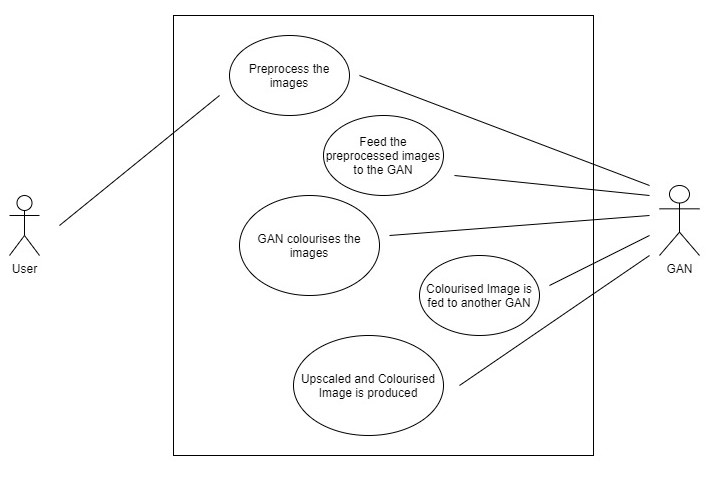
\includegraphics[width=\textwidth]{figures/use.jpg}}
	  \caption{Use case diagram}
	  \label{fig:usecase}
	\end{figure}
\end{center}

\section{Data Model and Description}
\subsection{Data Description}
Data objects that will be managed/manipulated by the software are described in this section. The database entities or files or data structures  required to be described. For data objects details can be given as below
\subsection{Data objects and Relationships}
  Data objects and their major attributes and relationships among data objects are described using an ERD- like form.



\section{Functional Model and Description}
A description of each major software function, along with data flow (structured analysis) or class hierarchy (Analysis Class diagram with class description for object oriented system) is presented.
\subsection{Data Flow Diagram}
\subsubsection{Level 0 Data Flow Diagram}
\subsubsection{Level 1 Data Flow Diagram}

\subsection{Description of functions}
A description of each software function is presented. A processing narrative for function n is presented.(Steps)/ Activity Diagrams. For Example Refer \ref{fig:act-dig}



\begin{center}
	\begin{figure}[!htbp]
		\centering
		\fbox{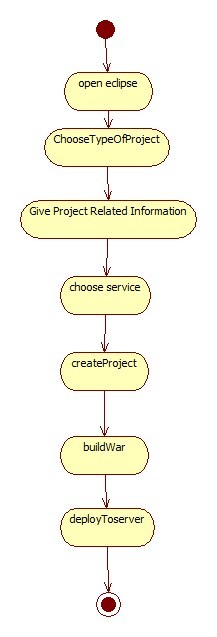
\includegraphics[height=430pt]{activity-dig.jpg}}
	  \caption{Activity diagram}
	  \label{fig:act-dig}
	\end{figure}
\end{center}




\subsection{Activity Diagram:}
\begin{itemize}
	\item	The Activity diagram represents the steps taken.
\end{itemize}

\subsection{Non Functional Requirements:}
\begin{itemize}
	\item	Interface Requirements
	\item	Performance Requirements
    \item	Software quality attributes such as availability [ related to Reliability], modifiability [includes portability, reusability, scalability] ,  		performance, security, testability and usability[includes self 			adaptability and user adaptability]
\end{itemize}

\subsection{State Diagram:}
  State Transition Diagram\\
Fig.\ref{fig:state-dig} example shows the state transition diagram of Cloud SDK. The states are
represented in ovals and state of system gets changed when certain events occur. The transitions from one state to the other are represented by arrows. The Figure    shows important states and events that occur while creating new project.

\begin{center}
	\begin{figure}[!htbp]
		\centering
		\fbox{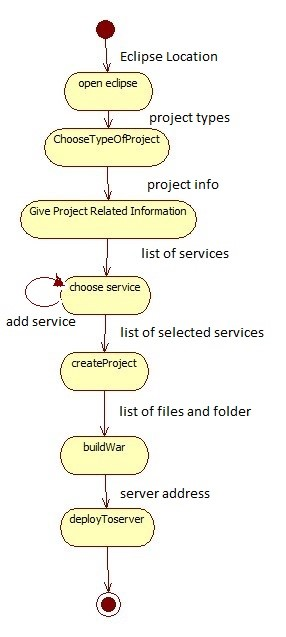
\includegraphics[width=230pt]{state-dig.jpg}}
	  \caption{State transition diagram}
	  \label{fig:state-dig}
	\end{figure}
\end{center}

 \subsection{Design Constraints}
Any design constraints that will impact the subsystem are noted.
 \subsection{Software Interface Description}
The software interface(s)to the outside world is(are) described.
The requirements for interfaces to other devices/systems/networks/human are stated.



\chapter{Detailed Design Document }
 \section{Introduction}
The project is largely inspired by Christian Ledig's SRGAN paper \cite{ledig2017photorealistic} and Dong et. al \cite{dong2014super} implementation of SRGANs using Tensorflow. Dahl et. al \cite{dahl2016automatic} introduction of residual encoding using VGG architecture and adaptation of GANs as conditional GANs by Mirza et al. \cite{mirza2014conditional} proved to be quite effective for implementing colorization of images. We provide detailed architectural design for each respective GANs and other networks that it will be compared with.
\section{Architectural Design}
	Generative Adversarial Networks (GANs) have two competing neural network models. The generator takes in the input and generates fake images. The discriminator gets the image from both the generator and the label along with the grayscale image and it determines which pair contains the real colored image. During training, the generator and the discriminator are playing a continuous game. At each iteration, generator can produce more realistic photo, while the discriminator is getting better at distinguishing fake photos. Both models are trained together in a minimax fashion and the goal is to train a generator to be indistinguishable from the real data.
	\subsection{Image Colorization}
	\hspace{0.4 in}With conditional GAN, both generator and discriminator are conditioning on the input $x$. Let the generator be parameterized by $\theta_g$ and the discriminator be parameterized by $\theta_d$. The minimax objective function can be defined as:
	\[
		\min_{\theta_g}\max_{\theta_d}\Big[\mathbb{E}_{x,y\sim p_{data}} \log D_{\theta_d}(x,y) + E_{x\sim p_{data}} \log(1 - D_{\theta_d}(x, G_{\theta_g}(x))\Big]
	\]

	Where, $G_{\theta_{g}}$ is the output of the generator and $D_{\theta_d}$ is the output of the discriminator.
	We're currently not introducing any noise in our generator to keep things simple for the time being. Also, we consider $L1$ difference between input $x$ and output $y$ in generator. On each iteration, the discriminator would maximize $\theta_d$ according to the above expression and generator would minimize $\theta_g$ in the following way:
	\[
		\min_{\theta_g}\Big[-\log(D_{\theta_d}(x,G_{\theta_g}(x)))+\lambda \Vert G_{\theta_g}(x) - y \Vert_1 \Big]
	\]

	With GAN, if the discriminator considers the pair of images generated by the generator to be a fake photo (not well colored), the loss will be back-propagated through discriminator and through generator. Therefore, generator can learn how to color the image correctly. At the final iteration, the parameters $\theta_g$ will be used in our generator to color grayscale images.

  \begin{center}
	\begin{figure}[!htbp]
		\centering
		\fbox{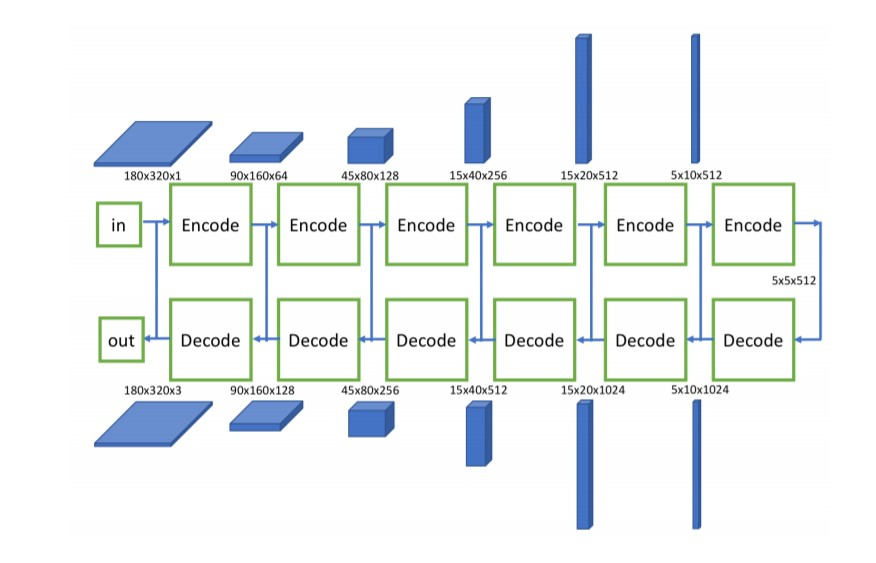
\includegraphics[width=\textwidth]{figures/encoder_decoder_generator_color.jpg}}
	  \caption{Encoder-Decoder ConvNets in Generator}
	  \label{fig:gen_color-dig}
	\end{figure}
\end{center}

  \begin{center}
	\begin{figure}[!htbp]
		\centering
		\fbox{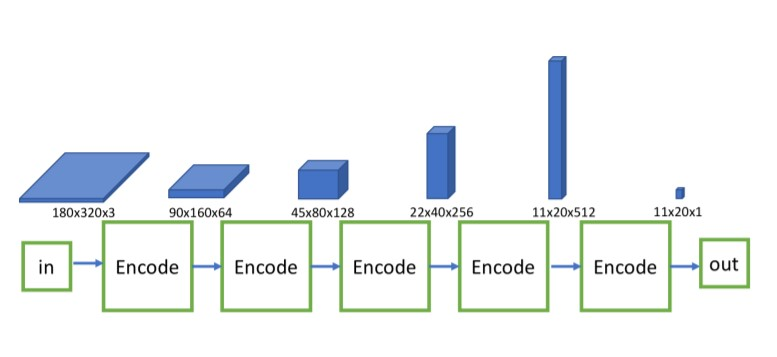
\includegraphics[width=\textwidth]{figures/discriminator_color.jpg}}
	  \caption{Discriminator}
	  \label{fig:disc_color-dig}
	\end{figure}
  \end{center}

\pagebreak

  \subsection{Image Super-resolution}
\hspace{0.4 in}We use the SRResNet as the generator in the SRGAN model as used by Ledig et. al \cite{ledig2017photorealistic}. It contains both the residual blocks and the skip connections, as seen in Figure \ref{fig:srgan-dig}. Within each residual block, there are two convolution layers followed by a Batch Normalization layer and a parametric ReLU layer. Finally, the image is then upscaled 4 times using two sub-pixel convolution layers \cite{shi2016subpixel}.
	\begin{center}
	\begin{figure}[!htbp]
		\centering
		\fbox{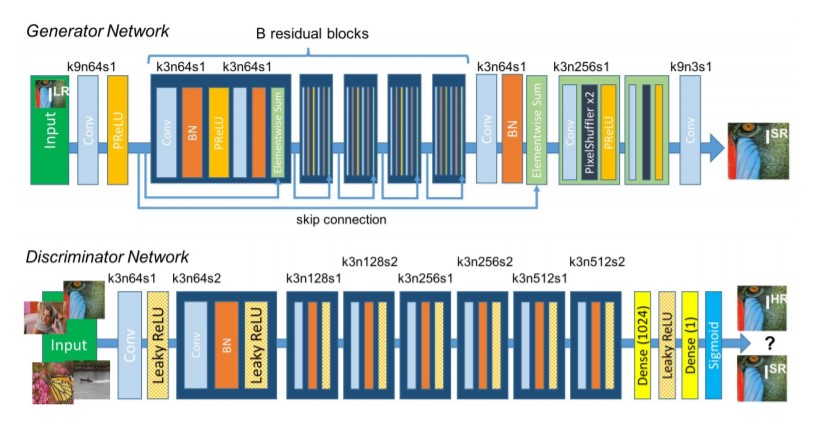
\includegraphics[width=\textwidth]{figures/ledig_srgan_architecture.jpg}}
	  \caption{SRGAN model: SRResNet generator and discriminator}
	  \label{fig:srgan-dig}
	\end{figure}
  \end{center}
  The generator's goal is to produce high resolution images to fool the discriminator of the GAN into thinking that it is receiving real instead of fake images. On the other hand the discriminator's goal is to classify the images it has received as either real images or generated images from the generator. The GANs objective function is a minimax game as mentioned in the previous section. We define the minimax function for this task with trivial changes in notation and express it as:

\[
		\min_{\theta_g}\max_{\theta_d}\mathbb{E}_{I^{HR}\sim p_{train}(I^{HR})}\big[ \log D_{\theta_d}(I^{HR})\big] + \mathbb{E}_{I^{LR}\sim p_{g}(I^{LR})}\big[\log(1 - D_{\theta_d}(G_{\theta_g}(I^{LR})))\big]
	\]
	where, $I^{HR}p_{train}(I^{HR})$ are the high resolution images. $I^{LR}p_g(I^{LR})$ are the input low resolution images, $G_{\theta_g}$ is the output of the generator and $D_{\theta_d}$ is the output of the discriminator. We use the perpetual loss function for VGG based content losses introduced by Ledig et. al \cite{ledig2017photorealistic} which is a weighted sum of a content loss $l^{SR}_X$ and an adversarial loss component $(10^{-3}l^{SR}_{Gen})$.

	For the content loss, we aim to use the VGG loss introduced by Ledig et. al\cite{ledig2017photorealistic} which is the euclidean distance between the feature representations of a reconstructed image $G_{\theta_g}(I^{LR})$ and the reference image $I^{HR}$:
	$$
		l^{SR}_{VGG_{i,j}} = \frac{1}{W_{i,j}H_{i,j}} \sum_{x=1}^{W_{i,j}}\sum_{y=1}^{H_{i,j}}\big(\phi_{i,j}(I^{HR})_{x,y}-\phi_{i,j}(G_{\theta_g}(I^{LR}))_{x,y}\big)^2
	$$
	where $W_{i,j}$ and $H_{i,j}$ represent the dimensions of the respective feature maps within VGG19 network. The adversarial generative loss $l^{SR}_{Gen}$ is defined on the probabilities of the discriminator $D_{\theta_d}(G_{\theta_g}(I^{LR}))$ over all the training samples as:
	$$
		l^{SR}_{Gen} = \sum_{n=1}^{N} - \log D_{\theta_d}(G_{\theta_g}(I^{LR}))
	$$

	$D_{\theta_d}(G_{\theta_g}(I^{LR}))$ is the probability that the reconstructed image $G_{\theta_g}(I^{LR}))$ is a natural HR image. For beter gradient behavior, we minimize $-\log D_{\theta_d}(G_{\theta_g}(I^{LR}))$ instead of $\log \big[1-D_{\theta_d}(G_{\theta_g}(I^{LR}))\big]$.

 \chapter{Dataset and Experimental setup}
Initially, we started by scraping the data off Hubble Legacy Archive. Using puppeteer(headless chrome), we scraped off hundreds of thousands of colorized images it has available. The Hubble Legacy archive is slow and produces grainy images with lots of noise and unprocessed images. A filter for M101 (Messier 101) galaxy rendered more than 80 thousand images with a 1 degree difference between consecutive right ascension. The data is large and has no particularly efficient way to clean without human investment. Cleaning tens of thousands of images by handpicking noiseless and well colored images is time consuming. For training the SRGAN, we need high resolution, well colored images. \\ \\
To that end, we scraped the Hubble Heritage project instead. The Hubble Heritage project releases the highest-quality astronomical images. They are all stitched together, colorized and processed to eliminate noise. Hubble Heritage then selects the best, most striking of these for public release. However, there are only $\sim150$ of these images that are actually useful. To increase the amount of data we had, we scraped images from the main Hubble website as well. This provided an extra approximately $\sim1000$ images.
Each image is a JPG image with dimensions of $256\times 256$ pixels and contains 3 channels of RGB.

 \chapter{Summary and Conclusion}
 \section{Summary}
 Low Resolution and Black and White Images in the Hubble Legacy Archive lie dormant and are needed to be upscaled and colourized for better visual discernment of the astromers. Images are initially scraped from the Hubble Legacy Arhive and the Hubble Legacy Project and a dataset is formed which is cleaned manually and is then fed to two Generative Adversarial Networks consecutively. The images of size ($64\times 64\times 1$) are initially colorized using a first GAN and an output image of size ($64\times 64\times 3$) with three RGB channels is obtained. This is then upscaled to a size of ($(64\cdot n)\times (64\cdot n)\times 3$). The output images are visually superior as well as colorized. These images are expected to be of greater use for astronomers than the older ones.

\section{Conclusion}
The images are upscaled and colourized using a completely automated algorithm which uses Deep Learning. Generative Adversarial Networks are  successfully used for the implementation and the images obtained are in public forum to be used for research, it is anticipated that this will aid the astronomers vastly in their efforts.

\bibliographystyle{ieeetr}
\bibliography{biblo}


\begin{appendices}


% \chapter{ALGORITHMIC DESIGN}
\chapter{Mathematical Model}











\chapter{Plagiarism Report }


\chapter{Paper Published (if any)}

\chapter{Sponsorship detail (if any)}



\end{appendices}


\end{document}
